% begin module limit-at-infinity-intro
\begin{frame}
\frametitle{Limits at Infinity; Horizontal Asymptotes}
\psset{xunit=0.85cm, yunit=0.85cm}
\begin{pspicture}(-7,-1.2)(7,1.6) \psaxes[ticks=none, labels=none]{<->}(0,0)(-6.5,-1.2)(6.5,1.5)
\psline(1,-0.1)(1, 0.1)
\rput[tl](1, -0.15){$1$}
\psplot[linecolor=red, plotpoints=1000]{-7}{7}{-1 x 2 exp add 1 x 2 exp add div }
\rput[tr](-1.1, -0.5){$y=\frac{x^2-1}{x^2+1}$}
\psline[linecolor=blue, linestyle=dashed](-7, 1)(7, 1)
\rput[lb] (0.5, 1.1){$y=1$}
\end{pspicture} 
%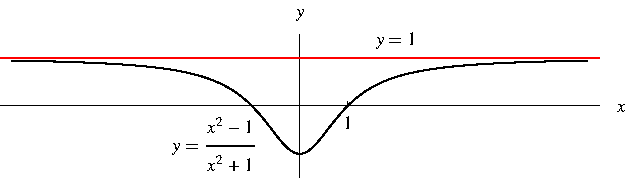
\includegraphics[width=12cm]{curve-sketching/pictures/04-04-intro.pdf}%
\begin{columns}[c]
\column{.3\textwidth}
\uncover<2->{%
\[
\begin{array}{|r|r@{}l|}
\hline
x & & \ \ f(x)\\
\hline
0 & - & 1\\
  \pm 1 &  & 0\\
  \pm 2 &  & 0.600000\\
  \pm 3 &  & 0.800000\\
  \pm 4 &  & 0.882353\\
  \pm 5 &  & 0.923077\\
 \pm 10 &  & 0.980198\\
%\pm 100 &  & 0.999800\\
\hline
\end{array}
\]
}%
\column{.7\textwidth}
\begin{itemize}
\item  Consider $f(x) = \frac{x^2-1}{x^2+1}$ as $x$ becomes large.
\item<2->  The values of $f(x)$ get closer and closer to $1$.
\item<3->  We express this by writing $\lim\limits_{x\to \infty} f(x) = 1$.
\item<4->  When $x$ is large negative, $f(x)$ is also near $1$.
\item<5->  We express this by writing $\lim\limits_{x\to -\infty} f(x) = 1$.
\end{itemize}
\end{columns}
\end{frame}
% end module limit-at-infinity-intro
